\documentclass[11pt]{article}

% ACL style: "review" (anonymous) -> "preprint" (names, page numbers) -> "final"
\usepackage[review]{acl}

\usepackage{times}
\usepackage{latexsym}
\usepackage[T1]{fontenc}
\usepackage[utf8]{inputenc}
\usepackage{microtype}
\usepackage{inconsolata}
\usepackage{amsmath}
\usepackage{amssymb}
\usepackage{booktabs}
\usepackage{multirow}
\usepackage{array}
\usepackage{tabularx}
\usepackage{xcolor}
\usepackage{url}
\usepackage{tikz}
\usetikzlibrary{positioning,arrows.meta}

\newcommand{\system}{\textsc{GNN-Pruner}}
\newcommand{\coarse}{\textsc{CoarseGNN}}
\newcommand{\fine}{\textsc{FineGNN}}
\newcommand{\rulepipe}{\textsc{Rule}}

\title{GNN-Pruner: Structure-Aware Graph Pruning for Grounded Question Answering\\ over Very Long Documents}

% ---- Review version (anonymous) ----
\author{Anonymous ACL Submission}

% ---- Preprint / final version: replace the line above with this block ----
% \author{
%   First Author \\ Affiliation \\ \texttt{email@domain} \And
%   Second Author \\ Affiliation \\ \texttt{email@domain} \And
%   Third Author \\ Affiliation \\ \texttt{email@domain} \And
%   Fourth Author \\ Affiliation \\ \texttt{email@domain}
% }

\begin{document}
\maketitle

% ======================================================================
\begin{abstract}
Answering questions over very long documents---contracts, reports, books---is limited by model context windows, by the cost of sending every token, and by models missing evidence placed deep in long inputs. We present \system{}, a system that prunes a document's own structure graph \emph{before} the language model is called, so that the model sees a small, dependency-aware, citable evidence pack. Documents are parsed into a four-layer graph (sections, sub-sections, paragraphs, sentences) with hierarchical, sequential, cross-reference and definition edges. A typed GraphSAGE model trained without hand labels (weak ``Silver Path'' supervision and a PPO keep policy) scores paragraph super-nodes; a second GNN scores sentences inside the kept paragraphs; windowed and global cross-edge attention targets cross-chapter evidence; and scoring can be distributed with exact parity. On a single 8\,GB laptop CPU, evidence packs stay at roughly 300--400 tokens from 100 to 10,000 pages (0.007\% of a 5M-token document), two-stage coarsening processes about 90\% fewer nodes at a cost of about one MRR point, and a 10,000-page question takes 4.7\,s, about 35$\times$ faster than a structured rule-based baseline. The GNN is the best ranker in its training domain but second to the rule-based baseline on real contracts, which we trace to domain shift. On a new nested long-document benchmark built from real contracts (CUAD) and novels (NarrativeQA), the pipeline retrieves every planted single and two-hop fact in a 9,988-page library from about 285 tokens, where dense retrieval at the same budget finds 39\% and 0\%. With an LLM answering only from the pack, every number in the reference answers of both test sets is stated correctly and required clauses are cited with recall 0.99--1.0. We report where the system falls short as carefully as where it works.
\end{abstract}

% ======================================================================
\section{Introduction}

Legal contracts, regulatory filings and long books routinely run to hundreds or thousands of pages. A 10,000-page document is about five million tokens, beyond the context window of any current language model. Even when a document fits, cost grows with every token sent, and models are less reliable at using evidence placed in the middle of long inputs \citep{liu2024lost,hsieh2024ruler}; whether to retrieve or to read everything remains an open trade-off \citep{xu2024retrievallong,li2024selfroute}. In professional use an answer must also come with its source: commercial legal research tools still produce unsupported answers \citep{magesh2024hallucination}, and an unsupported answer about a liability cap is not usable.

Retrieval-augmented generation (RAG) \citep{lewis2020rag,izacard2021fid} sends only the most similar chunks to the model, but flat chunking ignores what makes documents like contracts readable: their structure. A clause depends on the definitions it uses and on the provisions it cites (``subject to Section 4.2''); the answer to a question may sit in two chapters; and the most similar chunk is often not the one that answers. Recent work navigates summary trees \citep{sarthi2024raptor,chen2023memwalker,pageindex2025}, builds entity graphs \citep{edge2024graphrag,gutierrez2024hipporag}, or coordinates agents over chunks \citep{zhang2024chainofagents}; these rely on model-generated summaries, entities or reading for indexing or navigation.

\system{} takes a different route: it uses the document's \emph{native} structure graph and learns to prune it, so that the language model receives a small evidence pack that keeps the dependencies an answer needs. Our contributions are:
\begin{enumerate}
  \item \textbf{A complete structure-aware pruning system}: parsing to a four-layer graph; weakly supervised GNN scoring (Silver Paths, listwise training, a PPO keep policy); two-stage coarse-to-fine scoring; local and global cross-edge attention; distributed scoring with exact parity; dependency-aware merging; topology-routed prompts; and grounded answers with verified citations.
  \item \textbf{Measurements on commodity hardware from 100 to 10,000 pages}, including what does not work: the GNN's in-domain gains do not transfer to real contracts (domain shift), cross-chapter attention helps only in domain, and distribution gives exact results but little speed-up on one machine.
  \item \textbf{A nested long-document benchmark} (130 / 977 / 8,619-page contract data rooms from CUAD; 119 / 1,001 / 9,988-page libraries from NarrativeQA) with planted single, two-hop, distractor and absent facts, and an equal-evidence-budget comparison against dense retrieval.
  \item \textbf{Grounded answering}: an LLM answers only from the pack, every citation is checked, and we find that the model's own ``insufficient evidence'' judgement abstains more accurately than a score-based pre-check.
\end{enumerate}

% ======================================================================
\section{Related Work}

\paragraph{Long-context models.} Sparse and blockwise attention \citep{beltagy2020longformer,zaheer2020bigbird,liu2024ringattention} and recurrent memory \citep{bulatov2022rmt} let models read more, but long-document benchmarks \citep{shaham2022scrolls,bai2024longbench} and stress tests \citep{liu2024lost,hsieh2024ruler,kuratov2024babilong} show that effective use of long contexts lags the nominal window, and every token still costs. Direct comparisons find retrieval competitive with long contexts at a fraction of the cost \citep{xu2024retrievallong,li2024selfroute}. We instead reduce what the model reads.

\paragraph{Retrieval and graph-based RAG.} RAG \citep{lewis2020rag,izacard2021fid,asai2024selfrag} retrieves passages with sparse \citep{robertson2009bm25}, dense \citep{karpukhin2020dpr,reimers2019sbert} or late-interaction \citep{khattab2020colbert,santhanam2022colbertv2} retrievers, often fused \citep{cormack2009rrf}. Graph-based RAG builds and traverses graphs of entities or communities \citep{edge2024graphrag,gutierrez2024hipporag,peng2024graphragsurvey}, and GNN-RAG uses a GNN to retrieve over knowledge graphs \citep{mavromatis2025gnnrag}. Our graph is the document's own section, reference and definition structure, built without a language model.

\paragraph{Context compression.} Prompt compression drops low-information tokens with a small language model \citep{jiang2023llmlingua,jiang2024longllmlingua}, and RECOMP compresses retrieved documents into summaries \citep{xu2024recomp}. These operate on retrieved text and use a language model to compress it; we select whole document units by structure, without one, and keep them verbatim so they can be cited.

\paragraph{Trees and agents for long documents.} RAPTOR clusters and summarises text into a tree \citep{sarthi2024raptor}; MemWalker and PageIndex let a model navigate a summary tree \citep{chen2023memwalker,pageindex2025}; ReadAgent pages through a document with gist memories \citep{lee2024readagent}; Chain-of-Agents passes information between worker agents over chunks \citep{zhang2024chainofagents}. These rely on model calls for indexing or navigation; \system{} prunes with small learned scorers and calls the model once, on the pruned pack.

\paragraph{Graph neural networks for documents.} Graph convolution and attention \citep{kipf2017gcn,velickovic2018gat,hamilton2017graphsage} and relational variants with typed edges \citep{schlichtkrull2018rgcn} underlie question answering over knowledge and document graphs \citep{yasunaga2021qagnn,fang2020hgn}. Hierarchical pooling learns to coarsen graphs \citep{ying2018diffpool,gao2019graphunets}; we instead coarsen along the document's own paragraph structure, which keeps every kept unit citable. We use a four-layer hierarchy for pruning very long single documents, with coarse-to-fine scoring and cross-chapter attention.

\paragraph{Legal documents and grounded answers.} Contract understanding has been studied through clause extraction \citep{hendrycks2021cuad}, contract-level inference \citep{koreeda2021contractnli} and legal benchmarks \citep{chalkidis2022lexglue,guha2023legalbench}. Answer attribution asks models to cite their sources \citep{gao2023alce}, and abstaining on unanswerable questions \citep{rajpurkar2018squad2} relates to how well models know what they know \citep{kadavath2022know}.

\paragraph{Graph partitioning and distribution.} Partition-based GNN training splits graphs into clusters \citep{chiang2019clustergcn}. We partition with METIS \citep{karypis1998metis} or contiguous tree cuts and run scoring workers on Ray \citep{moritz2018ray}, replicating boundary nodes so each worker can score locally.

% ======================================================================
\section{Method}

\begin{figure}[t]
\centering
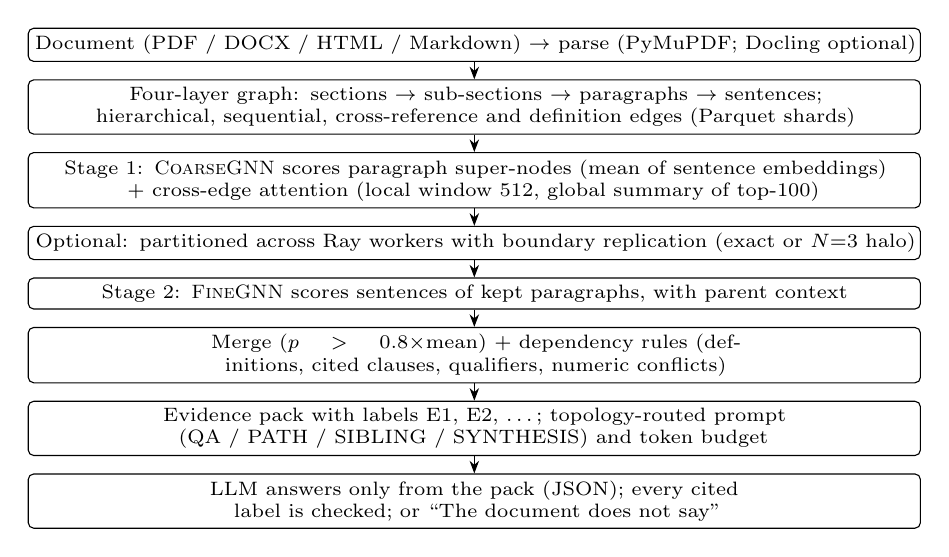
\begin{tikzpicture}[
  box/.style={draw, rounded corners=2pt, align=center, font=\scriptsize, text width=0.92\columnwidth, inner sep=2.5pt},
  node distance=2.2mm]
\node[box] (p) {Document (PDF / DOCX / HTML / Markdown) $\rightarrow$ parse (PyMuPDF; Docling optional)};
\node[box, below=of p] (g) {Four-layer graph: sections $\rightarrow$ sub-sections $\rightarrow$ paragraphs $\rightarrow$ sentences;\\ hierarchical, sequential, cross-reference and definition edges (Parquet shards)};
\node[box, below=of g] (c) {Stage 1: \coarse{} scores paragraph super-nodes (mean of sentence embeddings)\\ + cross-edge attention (local window 512, global summary of top-100)};
\node[box, below=of c] (d) {Optional: partitioned across Ray workers with boundary replication (exact or $N{=}3$ halo)};
\node[box, below=of d] (f) {Stage 2: \fine{} scores sentences of kept paragraphs, with parent context};
\node[box, below=of f] (m) {Merge ($p > 0.8\times$mean) + dependency rules (definitions, cited clauses, qualifiers, numeric conflicts)};
\node[box, below=of m] (r) {Evidence pack with labels E1, E2, \dots; topology-routed prompt (QA / PATH / SIBLING / SYNTHESIS) and token budget};
\node[box, below=of r] (a) {LLM answers only from the pack (JSON); every cited label is checked; or ``The document does not say''};
\foreach \u/\v in {p/g,g/c,c/d,d/f,f/m,m/r,r/a} \draw[-{Stealth[length=1.6mm]}] (\u) -- (\v);
\end{tikzpicture}
\caption{The \system{} pipeline. All scoring before the final answer runs without a language model.}
\label{fig:pipeline}
\end{figure}

Figure~\ref{fig:pipeline} shows the pipeline.

\subsection{Document graph}
Documents are parsed with PyMuPDF (layout heuristics, header/footer removal) or Docling \citep{auer2024docling}; both give identical end-to-end results on our test contracts in four formats. Each document becomes a four-layer directed acyclic graph: L1 section headings, L2 sub-section headings, L3 paragraphs / clauses / tables, L4 sentences or enumerated sub-clauses. A paragraph without sentence children receives one \emph{virtual} L4 node so that every path has the same depth. Edges are hierarchical, sequential (reading order within a layer), cross-reference (``Section 4.2'', ``clause 2(c)'') and definition (a use of a defined term $\rightarrow$ its definition). A 1,000-page document yields 51,304 nodes (parsed in 1.2\,s); 10,000 pages yield 510,486 nodes (12.6\,s). Graphs are stored as memory-mapped Parquet shards. Nodes are embedded with \texttt{all-MiniLM-L6-v2} \citep{wang2020minilm,reimers2019sbert}.

\subsection{Weak supervision: Silver Paths}
Training labels come without annotation, following the use of unsupervised rankers as weak supervision for neural ranking \citep{dehghani2017weak}. For each training question we take the top-10 sentence leaves from BM25 \citep{robertson2009bm25} and dense retrieval and walk up to their ancestors, which form a positive path set with graded relevance. Fusing the two rankings with equal-weight reciprocal rank fusion \citep{cormack2009rrf} let BM25's near-random order on paraphrased questions push the dense hits out of the top 10. We therefore weight BM25 by its term coverage $c$ of the question and dense retrieval by $1-c$, which raised paraphrase leaf recall on the training corpus from 0.54 to 0.96. Against known answers, silver leaf recall is 0.94 (train) and 0.96 (validation).

\subsection{\coarse{}: typed GraphSAGE}
Node features combine the paragraph embedding, its element-wise product with the question embedding, cosine similarity, BM25, term coverage and structural features; without the question features the model cannot rank at all (Table~\ref{tab:ablation}). With $\mathbf{h}^{(0)}_v = \mathrm{ReLU}(\mathbf{W}_{\mathrm{in}}\mathbf{x}_v)$, each of $L{=}2$ layers averages one GraphSAGE convolution \citep{hamilton2017graphsage} per edge type $t \in T$, in the spirit of relational GNNs \citep{schlichtkrull2018rgcn}:
\begin{align}
\mathbf{m}^{(k)} &= \tfrac{1}{|T|}\textstyle\sum_{t\in T}\mathrm{SAGE}_t\big(\mathbf{h}^{(k)}, E_t\big)\\
\mathbf{h}^{(k+1)} &= \mathrm{LN}\big(\mathbf{h}^{(k)} + \mathrm{Drop}(\mathrm{ReLU}(\mathbf{m}^{(k)}))\big)
\end{align}
The score reads both the input and the final representation (a skip connection): $s_v = \mathbf{w}^\top[\mathbf{h}^{(0)}_v; \mathbf{h}^{(L)}_v]$. Hidden size is 128. Training minimises a listwise cross-entropy \citep{cao2007listnet} between the softmax of scores over a document's paragraphs and a target distribution obtained from the silver grades with temperature $\tau{=}0.1$. A keep / prune policy is then fine-tuned with PPO \citep{schulman2017ppo} to retain answers at a small kept share; the supervised model remains the ranker.

\subsection{Coarse-to-fine scoring}
Paragraph super-nodes are the mean of their sentences' embeddings. Stage 1 keeps paragraphs with probability above $\theta$ times the mean ($\theta{=}1$), capped at the top 20\% (minimum 5); an optional absolute cap of 200 paragraphs bounds stage 2 on very long documents. Stage 2 (\fine{}) runs a two-layer GraphSAGE over the sentences of kept paragraphs; each sentence receives its parent's context through a projection scaled by a trainable $\alpha$ (initialised at 0.3), and the parent's stage-1 probability is an input feature. Sentences with probability above 0.8 times the mean are merged into the evidence set.

\subsection{Cross-edge attention}
To reach evidence in other chapters, node states attend within a 512-position window in document order (exact band attention, computed in blocks), and a global summary $\mathbf{g}$---the mean hidden state of the top-100 nodes---is broadcast to all nodes. The final score is $s_v + \mathrm{head}(\mathbf{a}_v) + \beta\,\sigma(\cos(\mathbf{a}_v,\mathbf{g}))$, where $\mathbf{a}_v$ is the attended state; the correction head starts at zero. Attention is trained with the GNN frozen, then jointly.

\subsection{Distributed scoring}
For very large graphs, coarse scoring is partitioned into contiguous chapter blocks (tree cut) or METIS parts \citep{karypis1998metis} and run on Ray actors \citep{moritz2018ray}. Each shard carries replicated boundary nodes (a \emph{halo}): either the last/first $N{=}3$ nodes at each edge, or an \emph{exact} halo covering the attention window and the 2-hop GNN neighbourhood. The only cross-shard data are three normalisation statistics and the global summary vector; an aggregator applies the keep rule, stage 2, merging and boundary stitching.

\subsection{Evidence pack and grounded answers}
After merging, dependency rules add what kept items need: definitions of terms they use, clauses they cite, qualifiers and continuations, and flags for conflicting numbers. The pack's topology selects a prompt template---SYNTHESIS when more than two clause citations link kept items, SIBLING when more than three items share a section, PATH when depth exceeds three, otherwise QA---and a per-route token budget (250--300 evidence tokens). The language model receives only the labelled items (E1, E2, \dots) and returns JSON with an answer, cited labels, a confidence and an ``insufficient'' flag. Every cited label must exist in the pack; quoted citations are mapped back to items; unanswerable questions should yield ``The document does not say.''

% ======================================================================
\section{Experimental Setup}

\paragraph{Data.} Table~\ref{tab:data} lists the evaluation data. The two test sets were never used for tuning. GNN training uses a corpus of 48 generated contracts (985 pages; 1,060 training and 280 validation questions with known answer sentences); no generated sentence or question overlaps the test sets. Development sets are small sets of real contract questions used for thresholds and calibration.

\begin{table}[t]
\centering
\scriptsize
\setlength{\tabcolsep}{3pt}
\begin{tabular}{@{}llr@{}}
\toprule
\textbf{Set} & \textbf{Documents} & \textbf{Questions} \\
\midrule
test & 2 real contracts, $\leq$1 page & 40 \\
test-long & same, $\sim$10 pages each & 40 \\
dev & real contracts (4 sets) & 11--36 each \\
generated val & 10 generated contracts & 280 \\
scale & generated, 100--10,000 pp. & 8--12 per size \\
adversarial & 20 q.\ $\times$ 5 perturbations & 100 \\
\midrule
data rooms & CUAD, 130 / 977 / 8,619 pp. & 42 / 109 / 176 \\
libraries & NarrativeQA, 119 / 1,001 / 9,988 pp. & 42 / 94 / 200 \\
\bottomrule
\end{tabular}
\caption{Evaluation data. Each test set has 4 unanswerable questions; dev sets cover calibration, long documents, multi-passage and cross-chapter questions. The long-document benchmark (bottom; CUAD \citep{hendrycks2021cuad}, NarrativeQA \citep{kocisky2018narrativeqa}) nests each size inside the next; its questions are CUAD clause spans (and clauses CUAD marks absent), NarrativeQA human questions, and planted facts.}
\label{tab:data}
\end{table}

\paragraph{Long-document benchmark.} Contract data rooms concatenate real CUAD contracts (each a chapter); libraries concatenate NarrativeQA test-set novels from Project Gutenberg (each book a part). Sizes are nested (130 $\subset$ 977 $\subset$ 8,619 pages), so every question is asked at each size containing it. We plant facts at known positions: single facts with reworded questions and a look-alike distractor elsewhere; two-hop facts split across contracts or distant chapters; and questions about facts never planted. A page is 3,000 characters.

\paragraph{Systems.} \system{} (two-stage + attention, ``GNN''); the same without attention (``two-stage''); a no-coarsening variant (\fine{} over every node); and \rulepipe{}, a structured baseline we also built: a query planner, hybrid retrieval (BM25, phrase, dense, structural and graph sources fused by weighted RRF), bounded graph expansion, a 12-feature linear scorer, adaptive pruning and the same dependency rules. Single-signal baselines are BM25 and dense retrieval; on the long-document benchmark we add dense retrieval over $\sim$300-token title-prefixed chunks at top-1 (the pipelines' evidence budget) and top-5.

\paragraph{Metrics.} Ranking: MRR and hit@1 of the first answer paragraph; Recall@10. Evidence: whether the pack contains every gold span (word-3-gram coverage $\geq 0.5$ on the long-document benchmark). Answers: token F1 against the reference, whether every number in the reference appears, citation precision / recall, abstention on unanswerable questions and false abstention on answerable ones. Efficiency: latency p50 (p99), evidence tokens, build time, memory.

\paragraph{Hardware and models.} One MacBook, 8 CPU cores, 8\,GB RAM, no GPU. Answers use \texttt{gemini-3.1-flash-lite} through its free tier; the judge for clause answers is a different model \citep{zheng2023judge} (\texttt{gemini-3.1-flash-lite} judging \texttt{gemini-3.5-flash-lite} answers, Section~\ref{sec:longbench}).

% ======================================================================
\section{Results}

\subsection{Ranking and the domain gap}

\begin{table}[t]
\centering
\scriptsize
\setlength{\tabcolsep}{3pt}
\begin{tabular}{@{}lccccc@{}}
\toprule
\textbf{Set} & \textbf{BM25} & \textbf{Dense} & \textbf{\rulepipe{}} & \textbf{GNN} & \textbf{GNN-gold}$^*$ \\
\midrule
generated val & .633/.56 & .758/.65 & .776/.70 & \textbf{.794}/\textbf{.71} & .932/.89 \\
dev multi-passage & .636/.45 & .849/.73 & .864/.73 & \textbf{.955}/\textbf{.91} & .909/.82 \\
contracts (test) & .795/.72 & .859/.75 & \textbf{.965}/\textbf{.94} & .935/.89 & .908/.86 \\
contracts-long (test) & .725/.61 & .786/.69 & \textbf{.918}/\textbf{.86} & .852/.78 & .823/.78 \\
\bottomrule
\end{tabular}
\caption{Paragraph ranking, MRR / hit@1. $^*$Trained on known answers instead of Silver Paths: an upper bound on label noise, not the method.}
\label{tab:ranking}
\end{table}

Table~\ref{tab:ranking} shows the central finding. In its training domain the GNN is the best ranker, ahead of dense retrieval, BM25 and the rule-based pipeline, and it leads clearly on multi-passage development questions (MRR 0.955 vs 0.864). On the real test contracts it is second to the rule-based pipeline (0.935 vs 0.965; 0.852 vs 0.918 on long documents), though far ahead of BM25 and dense retrieval. A model trained on gold labels does no better on the test sets (0.908, 0.823), so the gap is not silver-label noise but domain shift: training contracts are templated. In domain, silver labels cost about 0.14 MRR relative to gold labels (0.79 vs 0.93). Recall@10 is 0.95--1.0 for the GNN on every set.

\begin{table}[t]
\centering
\scriptsize
\begin{tabular}{@{}lccc@{}}
\toprule
\textbf{Variant} & \textbf{gen. val} & \textbf{test} & \textbf{test-long} \\
\midrule
typed + skip (final) & .794 & .935 & .852 \\
typed, no skip & .799 & .921 & .881 \\
no edges (per-node MLP) & .780 & .919 & .835 \\
untyped GraphSAGE & .722 & .898 & .833 \\
no question input & .091 & .213 & .111 \\
\bottomrule
\end{tabular}
\caption{\coarse{} ablations (MRR). Run-to-run spread is about $\pm$0.01.}
\label{tab:ablation}
\end{table}

Table~\ref{tab:ablation} shows that edges help a little and typed edges more (untyped: $-$0.07 in domain), while the question input is indispensable. The PPO keep policy trades a little ranking quality (MRR $-$0.01 to $-$0.03) for retention: on long test documents it keeps 2.1\% of paragraphs while retaining 90.3\% of answers (supervised scores at a comparable share: 0.8\% / 76.4\%).

\subsection{Coarsening and scale}

\begin{table}[t]
\centering
\scriptsize
\setlength{\tabcolsep}{2.5pt}
\begin{tabular}{@{}llcccrr@{}}
\toprule
\textbf{Set} & \textbf{Method} & \textbf{MRR} & \textbf{h@1} & \textbf{Rec.} & \textbf{Share} & \textbf{Nodes} \\
\midrule
gen. val & 2-stage & .778 & .686 & .977 & 6.4\% & 92 \\
 & flat & .791 & .704 & 1.0 & 18.3\% & 795 \\
test & 2-stage & .887 & .806 & .889 & 13.0\% & 15 \\
 & flat & .891 & .833 & .958 & 19.7\% & 56 \\
test-long & 2-stage & .835 & .750 & .931 & 2.5\% & 63 \\
 & flat & .851 & .778 & 1.0 & 17.0\% & 620 \\
\bottomrule
\end{tabular}
\caption{Sentence-level ranking with two-stage coarsening and without it (flat): MRR, hit@1, answers in the merged set (Rec.), share of sentences merged, and nodes in the fine stage.}
\label{tab:coarsening}
\end{table}

Coarsening keeps quality close to single-pass scoring while processing about 90\% fewer nodes (Table~\ref{tab:coarsening}): 63 instead of 620 fine nodes on long test documents, at 0.4--1.6 MRR points below no coarsening on most sets. On long documents only 2.5\% of sentences are merged, with 93\% of answers kept; the evidence pack is 2.8\% of the document's words. End to end, the GNN path reaches evidence recall 0.986 / 0.958 on the two test sets without a query planner (rule-based: 1.0 / 1.0).

\begin{table}[t]
\centering
\scriptsize
\begin{tabular}{@{}rrccc@{}}
\toprule
\textbf{Pages} & \textbf{Nodes} & \textbf{Two-stage} & \textbf{+ cap 200} & \textbf{No coarsening} \\
\midrule
100 & 5,409 & 12 ms & 18 ms & 39 ms \\
1,000 & 51,459 & 198 ms & 72 ms & 574 ms \\
10,000 & 510,910 & 4.07 s & 1.34 s & out of memory \\
\bottomrule
\end{tabular}
\caption{Coarse + fine scoring latency (CPU); answer paragraphs kept and merged at every size.}
\label{tab:scale}
\end{table}

With the top-20\% keep rule the fine stage grows with the document (Table~\ref{tab:scale}); an absolute cap of 200 paragraphs makes it constant at no recall cost on these documents. The no-coarsening model could not run at 10,000 pages within 8\,GB: coarsening is what makes that size feasible on this machine.

\subsection{Cross-chapter evidence}

\begin{table}[t]
\centering
\scriptsize
\begin{tabular}{@{}lccc@{}}
\toprule
\textbf{Set ($n$)} & \textbf{No attention} & \textbf{Attention} & \textbf{\rulepipe{}} \\
\midrule
generated val (40) & .850 / .950 & \textbf{.917} / \textbf{1.00} & .700 \\
test (7) & 1.00 / .714 & 1.00 / .714 & 1.00 \\
test-long (7) & .714 / .714 & .714 / .762 & \textbf{1.00} \\
\bottomrule
\end{tabular}
\caption{Cross-chapter questions: paragraph complete@10 / stage-1 complete (attention: mean of 3 seeds); \rulepipe{} follows references explicitly.}
\label{tab:crosschapter}
\end{table}

In domain, attention raises cross-chapter complete@10 from 0.85 to 0.92 and stage-1 completeness from 0.95 to 1.00 in all three seeds (Table~\ref{tab:crosschapter}); local-only (0.900) and global-only (0.875) variants each recover part of the gain, and placing attention only at the fine stage helps least (0.850), since paragraphs are already chosen. On the real contracts the effect is within noise, and explicit reference following in the rule-based pipeline still wins on long documents (1.0 vs 0.71). At 1,000 pages attention adds about 0.3\,s of CPU time.

\subsection{Distributed scoring}

\begin{table}[t]
\centering
\scriptsize
\setlength{\tabcolsep}{3pt}
\begin{tabular}{@{}lcccc@{}}
\toprule
\textbf{Halo, workers} & \textbf{Replicated} & \textbf{Max $|\Delta|$ logit} & \textbf{Top-50 agree} & \textbf{Coarse stage} \\
\midrule
exact, 1 & 0\% & $6\times10^{-6}$ & 1.00 & 7.2 s \\
exact, 2 & 43\% & $7\times10^{-6}$ & 1.00 & 9.2 s \\
exact, 4 & 96\% & $7\times10^{-6}$ & 1.00 & 15.7 s \\
$N{=}3$, 2 & 0\% & 3.64 & 0.94 & 6.7 s \\
$N{=}3$, 4 & 0\% & 4.69 & 0.92 & 5.8 s \\
\bottomrule
\end{tabular}
\caption{Distributed scoring at 10,000 pages (tree cut, Ray on one 8-core machine). Single process: 7.6 s.}
\label{tab:distributed}
\end{table}

Exact halos reproduce single-process scores to within $7\times10^{-6}$ for 1--4 workers, with tree-cut and METIS partitions, at 1,000 and 10,000 pages (Table~\ref{tab:distributed}). A 3-node halo is not exact (logit drift up to 4.7) because a two-layer GNN reads two hops and headings and references cross shard edges, yet every answer was still kept. Exact parity is expensive for this graph shape: a heading links to all of its paragraphs, so a 2-hop halo pulls in whole neighbouring chapters. On one machine more workers buy little (best 1.3$\times$ on the coarse stage) because a single process already uses all cores; the measured benefit is memory per worker and a working protocol, while speed-ups require separate machines.

\subsection{End-to-end latency and tokens}

\begin{table}[t]
\centering
\scriptsize
\setlength{\tabcolsep}{3pt}
\begin{tabular}{@{}rccccc@{}}
\toprule
\textbf{Pages} & \textbf{Two-stage} & \textbf{GNN} & \textbf{\rulepipe{}} & \textbf{GNN pack} & \textbf{Share of doc.} \\
\midrule
100 & 23 ms & 53 ms & 60 ms & 372 tok & 0.72\% \\
1,000 & 165 ms & 463 ms & 1,517 ms & 394 tok & 0.08\% \\
10,000 & 4.7 s & 9.9 s & 167 s & 377 tok & 0.007\% \\
\bottomrule
\end{tabular}
\caption{End-to-end latency p50 per question (one CPU process) and evidence pack size. Rule-based packs: 266 / 324 / 300 tokens.}
\label{tab:latency}
\end{table}

Packs stay at about 300--400 tokens whatever the document size (Table~\ref{tab:latency}), so a 5.09M-token document is answered from 377 tokens, about 13,500$\times$ fewer than full context. At 10,000 pages the two-stage model is about 35$\times$ faster than the rule-based pipeline, whose index build also takes 6 minutes and 2.7\,GB. Cross-edge attention roughly doubles latency. Evidence recall on these generated scale documents is 1.0 / 0.88 / 0.83 for the GNN and 0.75 / 0.71 / 0.92 for the rule-based pipeline at 100 / 1,000 / 10,000 pages (12 questions each). For reference, the design specification we started from targeted 80\,ms at 10,000 pages on a four-GPU cluster; on one CPU we measure 4.7--9.9\,s.

\paragraph{Robustness.} On 100 perturbed questions (distractor topic, wrong number, swapped parties, typos, paraphrase), all systems keep Recall@10 at 0.99--1.0; the top-ranked passage is kept in 83\% (GNN), 88\% (two-stage) and 86\% (rule-based) of cases, with typos and party swaps hurting most.

\subsection{Grounded answers}
\label{sec:answers}

\begin{table}[t]
\centering
\scriptsize
\setlength{\tabcolsep}{2.5pt}
\begin{tabular}{@{}lccccc@{}}
\toprule
\textbf{System} & \textbf{F1} & \textbf{Numbers} & \textbf{Cit. P / R} & \textbf{Abstain} & \textbf{False abst.} \\
\midrule
\rulepipe{}, extractive (no LLM) & .35--.38 & .55--.60 & .85--.94 / .71--.79 & 5/8 & 5.6--8.3\% \\
\rulepipe{} + LLM, pre-check on & .46--.47 & 1.00 & .83 / 1.00 & 8/8 & 5.6--8.3\% \\
\rulepipe{} + LLM, model decides & .45--.47 & 1.00 & .83 / 1.00 & 8/8 & 0\% \\
GNN + LLM & .46--.47 & 1.00 & .86 / .99 & 8/8 & 0\% \\
\bottomrule
\end{tabular}
\caption{Answers on the two test sets (80 questions; ranges over the two sets). LLM: \texttt{gemini-3.1-flash-lite}, answering only from the pack.}
\label{tab:answers}
\end{table}

With a language model answering from the pack, every number in every reference answer is stated correctly and gold clauses are cited with recall 0.99--1.0 (Table~\ref{tab:answers}); no answer cites a label outside the pack. Token F1 rises only to 0.46--0.47 because answers are full sentences carrying conditions the short references omit. Citation precision of 0.83--0.86 mostly reflects definitions and conditions added by the dependency rules, which models cite but gold snippets do not list. A score-based retrieval-confidence check that refuses before the model is called wrongly refused 5 paraphrased questions; letting the model judge sufficiency refused all 8 unanswerable questions and no answerable one.

\subsection{Long-document benchmark}
\label{sec:longbench}

\begin{table}[t]
\centering
\scriptsize
\setlength{\tabcolsep}{2.5pt}
\begin{tabular}{@{}lcccc@{}}
\toprule
\textbf{Document (pages)} & \textbf{Dense k=1} & \textbf{\rulepipe{}} & \textbf{GNN} & \textbf{Dense k=5} \\
 & ($\sim$200 tok) & ($\sim$270 tok) & ($\sim$270 tok) & ($\sim$1.2k tok) \\
\midrule
data room (130) & .17 / .00 & .67 / .00 & \textbf{.83} / .00 & .67 / .00 \\
data room (977) & .17 / .00 & \textbf{.83} / .25 & \textbf{.83} / \textbf{1.00} & .42 / .00 \\
data room (8,619) & .11 / .00 & .39 / .67 & \textbf{.44} / \textbf{1.00} & .39 / .00 \\
library (119) & .67 / .00 & \textbf{1.00} / \textbf{1.00} & \textbf{1.00} / \textbf{1.00} & .67 / .00 \\
library (1,001) & .42 / .00 & \textbf{1.00} / \textbf{1.00} & \textbf{1.00} / \textbf{1.00} & .83 / .25 \\
library (9,988) & .39 / .00 & out of memory & \textbf{1.00} / \textbf{1.00} & .61 / .17 \\
\bottomrule
\end{tabular}
\caption{Planted facts found in the pack: single / two-hop (6--18 single and 2--6 two-hop questions per document).}
\label{tab:longbench}
\end{table}

At an equal evidence budget, the pipelines find planted facts far more often than dense retrieval (Table~\ref{tab:longbench}); dense retrieval catches up only partly with five times the text. In the 9,988-page library the GNN pipeline finds every planted single and two-hop fact from about 285 tokens. In data rooms of near-identical contracts, the pipelines fall from 0.83 at 977 pages to 0.39--0.44 at 8,619 pages: they find the right \emph{kind} of clause in the wrong contract, since distractors are the same clause type elsewhere. Real CUAD clauses are hard for every system at a small budget (evidence found: GNN 0.07--0.16, rule-based 0.13--0.14, dense top-1 0.13--0.20; dense top-5 0.37--0.60). At about 10,000 pages, the GNN pipeline needs 17--38 minutes to index, 3.1--3.5\,GB and 6.8--9.6\,s per question; the rule-based pipeline could not index the 9,988-page library within 8\,GB. With an LLM on the 130-page data room, sending the whole document (about 87k tokens) to a small model (\texttt{gemini-3.5-flash-lite}) answered 33\% of clause questions correctly by a model judge, the same as dense top-5 and above the rule-based pack (13\%), and missed half of the planted facts.

\subsection{Human evaluation}
In a blind A/B comparison of evidence packs from the GNN and rule-based pipelines on 20 test questions, rated by one author, preference was tied (6 / 6, 8 equal) and the preferred pack was sufficient to answer in all 20. In 11 of 12 decided pairs the shorter sufficient pack was chosen, which points to the token budget as the main lever.

% ======================================================================
\section{Discussion}

Three lessons stand out. First, \emph{structure is worth exploiting before the model reads}: constant-size packs that keep definitions and cited clauses make 10,000-page documents answerable from a few hundred tokens on a laptop. Second, \emph{learned scoring needs in-domain labels}: the GNN wins where it was trained and loses to explicit rules on real contracts, and the gold-label control shows that better synthetic labels would not close this gap; real-document supervision would. Third, \emph{explicit reference following remains strong}: on real contracts it beats learned cross-chapter attention, suggesting the two should be combined rather than one replacing the other.

% ======================================================================
\section{Limitations}

\begin{itemize}\setlength\itemsep{0pt}
\item \textbf{Domain shift.} The GNN is trained on generated contracts and trails a rule-based pipeline on real ones; real clause retrieval (CUAD) is weak for all systems at a small budget.
\item \textbf{Small evaluation sets.} The main test sets have 40 questions each and several settings have 7--20; we report no confidence intervals or significance tests \citep{dror2018hitchhiker}. Differences of a few points are within noise.
\item \textbf{Generated data.} Training documents, scale documents and planted facts are synthetic, although the long-document benchmark is built on real contracts and novels.
\item \textbf{No strong long-context baseline.} We compared against a small free model reading the whole document, not a frontier long-context model.
\item \textbf{Human evaluation.} One rater (an author) and 20 questions.
\item \textbf{Hardware.} All results are on one CPU laptop; distribution was not tested across machines, and GPU latency is not measured.
\item \textbf{Scope.} English contracts and novels; text PDFs only (no OCR); legal interpretation is out of scope and the system is not legal advice.
\end{itemize}

\section{Ethics Statement and Use of AI Assistants}
All datasets are publicly available under their licences (CUAD: CC BY 4.0; NarrativeQA: Apache 2.0; Project Gutenberg texts: public domain in the US); no personal data was collected. The system reports what documents say and abstains when evidence is missing; it is not a substitute for legal advice. An AI coding assistant was used to help implement the system and draft text; the authors designed the study, checked the code and verified every reported number against the recorded experiment logs.

% ======================================================================
\section{Conclusion}

\system{} prunes a document's own structure graph so that a language model answers from a small, dependency-aware, cited pack. On one laptop it keeps evidence at roughly 300--400 tokens from 100 to 10,000 pages, processes about 90\% fewer nodes through coarsening, answers 10,000-page questions in seconds, and retrieves every planted fact in a 9,988-page library at a budget where dense retrieval finds fewer than half. Its learned components help in their training domain and need real-domain supervision to beat explicit rules on real contracts. We release the code and the benchmark generator.

\bibliography{custom}

\end{document}
